%%%%%%%%%%%%%%%%%%%%%%%%%%%%%%%%%%%%%%%%%%%%%%%%%%%%%%%%%%%%%%%%%%%%%%%%%%%%%%%%%%%%%%%%%
%%                                                                                     %%
%%                This file is part of the CAPH Compiler distribution                  %%
%%                            http:%/caph.univ-bpclermont.fr                           %%
%%                                                                                     %%
%%                                  Jocelyn SEROT                                      %%
%%                         Jocelyn.Serot@univ-bpclermont.fr                            %%
%%                                                                                     %%
%%         Copyright 2011-2018 Jocelyn SEROT.  All rights reserved.                    %%
%%  This file is distributed under the terms of the GNU Library General Public License %%
%%      with the special exception on linking described in file ..%LICENSE.            %%
%%                                                                                     %%
%%%%%%%%%%%%%%%%%%%%%%%%%%%%%%%%%%%%%%%%%%%%%%%%%%%%%%%%%%%%%%%%%%%%%%%%%%%%%%%%%%%%%%%%%

\chapter{Using the caph compiler}
\label{cha:using-caph-compiler}

The \caph compiler can be used to
\begin{itemize}
\item obtain graphical (\texttt{.dot}) representations of program,
\item simulate programs or
\item generate SystemC or VHDL code.
\end{itemize}

This chapter describes how to invoke compiler on the command-line (on Unix systems). A separate
document describes the graphical IDE (running under MacOS and Windows platforms).

The compiler is invoked with a command like :

\begin{alltt}
caphc [options] file
\end{alltt}

where \texttt{file} is the name of the file containing the source code (by convention, this file
should be suffixed \texttt{.cph}). 

The complete set of options is described in App.~\ref{cha:compiler-options}.

The set of generated files depends on the selected target. The output file \texttt{caph.output}
contains the list of the generated file.

\section{Generating a graphical representation of the program}
\label{sec:gener-graph-repr}


\begin{example}
caphc -dot foo.cph  
\end{example}

The previous command generates a graphical representation of the program contained in file
\texttt{foo.cph} and writes it in file \texttt{foo.dot}.  This representation can be viewed with the
\texttt{Graphviz} suite of tools\footnote{Available freely from \texttt{http://www.graphviz.org}.}.

\section{Running the simulator}
\label{sec:running-simulator}

\begin{example}
caphc -sim -stop_after 200 foo.cph  
\end{example}

The previous command runs the program contained in file \texttt{foo.cph} for 200 execution cycles.

\section{Generating SystemC code}
\label{sec:gener-syst-code}

\begin{example}
caphc -systemc foo.cph  
\end{example}

The previous command generates the SystemC code corresponding the program contained in file
\texttt{foo.cph}. The following files are written :
\begin{itemize}
\item a file \texttt{foo\_expanded.dot}, containing a modified version of the program graphical
  description,  in which explicit flow-splitting boxes have been inserted,
\item a file \texttt{foo\_net.cpp}, containing the network description,
\item a pair of files \texttt{x\_act.h}, \texttt{x\_act.cpp} for each instance\footnote{If the actor
    is monomorphic, there will a single instance; otherwise there will be as many instances as
    distinct type and size specialisations of this actor. Each instance goes in a distinct pair of
    files. A name mangling mechanism is used to distinguish between files.}
  appearing in the program, containing respectively the interface and the implementation of the
  actor,
\item if some global constants and/or functions are defined, a pair of files \texttt{foo\_globals.h},
  \texttt{foo\_globals.cpp}, containing the C++ prototypes (resp. definitions) of the corresponding
  values. These files also contains the interface (resp. implementation) of the user defined variant
  types when such types have been declared in the program (see Sec.~{cha:variants-impl}),
\item if needed, a file \verb|foo_splitters.h| containing the interface and implementation of
  actors for performing $1 \rightarrow n$ flow replication.
\end{itemize}

The produced files can then compiled using the standard SystemC toolchain. When compiling
(resp. linking) the \caph-specific headers (resp. library) must be available\footnote{These headers
  and library are located in \texttt{\${CAPH}/lib/systemc} where \texttt{\${CAPH}} points to the
  installation directory of the \caph toolset.}. The easiest way to compile the generated code is to
use the \verb|-make| option of the compiler and to rely on the predefined skeleton makefile
\verb|$(CAPH)/lib/etc/Makefile.core| (see Sec.~\ref{sec:makefiles}.

\section{Generating VHDL code}
\label{sec:generating-vhdl-code}

\begin{example}
caphc -vhdl foo.cph  
\end{example}

The previous command generates the VHDL code corresponding the program contained in file
\texttt{foo.cph}. The following files are written :
\begin{itemize}
\item a file \verb|foo_expanded.dot|, containing a modified version of the program graphical
  description,  in which FIFO buffers and explicit flow-splitting boxes have been inserted,
\item a file \verb|foo_net.vhd|, containing the (structural) network description,
\item a file \verb|xxx_act.vhd| for each instance of actor \verb|xxx| appearing in
  the program, containing the interface and implementation of the actor,
\item if some global constants and/or functions are defined, a pair of files
  \verb|foo_globals.vhd|, containing the VHDL description of the corresponding values,
\item if the program declares some variant types, a file \verb|foo_types.vhd| containing the description
  of the VHDL package implementing the corresponding types\footnote{In case of polymorphic variants,
    there's one package per distinct monomorphic instanciation of the  declared type.},
\item if needed, a file \verb|foo_splitters.vhd| containing the interface and implementation of
  actors for performing $1 \rightarrow n$ flow replication,
\item a file \verb|foo_tb.vhd|, containing a \emph{test bench} for simulating the resulting
  design.
\end{itemize}

The produced files can then compiled, simulated and synthetized using a standard VHDL
toolchain\footnote{We use the Quartus II toolchain from Altera.}. When compiling
the \caph-specific \texttt{dc} library, containing the \texttt{dcflow} package, must be
available\footnote{This library, and the corresponding package(s) 
  and library are located in \texttt{\${CAPH}/lib/vhdl} where \texttt{\${CAPH}} points to the
  installation directory of the \caph toolset.}. 
 As with the SystemC backend, the easiest way to compile the generated code is to
use the \verb|-make| option of the compiler and to rely on the predefined skeleton makefile
\verb|$(CAPH)/lib/etc/Makefile.core| (see Sec.~\ref{sec:makefiles}.

\section{File I/O}
\label{sec:file-io}

When performing simulations of either using the reference interpreter or the generated SystemC code
input data streams and output streams are read from (resp. written to) text files.

For example, if the program contains the following lines :

\begin{lstlisting}
stream inp : signed<10> dc from "sample.txt";
stream res : unsigned<1> dc to "result.txt";
\end{lstlisting}

then the input stream will be read from file \verb|sample.txt| and the output stream written to file
\verb|result.txt|\footnote{In the directory from which the \caph compiler is invoked. Absolute and
  relative pathnames are also possible. }. 

\medskip
For streams containing values with a scalar type (see Sec.~\ref{sec:scalar-types}), these files will
simply contain the sequence of input (resp.output) tokens, separated by white space(s). For example,
here's the contents of a file containing eight tokens of type \verb|unsigned<8>| :

\begin{verbatim}
12 34 67 6 99 0 0 55
\end{verbatim}

\medskip
For streams containing values with an array type (see Sec.~\ref{sec:structured-types}), each array
will be denoted as a comma-separated list of values and enclosed between braces. For example, a file
describing a stream of four arrays of size 4 is :

\begin{verbatim}
{ 1,2,3,4 } { 10, 20, 30, 40 } { 100, 200, 300, 400 } { 1000, 2000, 3000, 4000 }
\end{verbatim}

\medskip
For streams containing values with a variant type (see Sec.~\ref{sec:structured-types}), each token
will denote, textually, either a nullary constructor or a n-ary constructor, followed by the
associated value(s).

For example, a file describing a stream of values with type \verb|unsigned<8> option| (as introduced in
Sec.~\ref{sec:type-declarations}), is~:

\begin{verbatim}
Absent Present 2 Present 4 Absent Absent Present 8
\end{verbatim}

\noindent
and  a file describing a stream of values with type \verb|(signed<8>,bool) pair| is~:

\begin{verbatim}
Pair 1 true Pair 8 false Pair 0 100
\end{verbatim}

In particular, input or input files representing streams structured with the \verb|t dc| type can be
denoted using the \verb|Data|, \verb|EoS| and \verb|SoS|
constructors. Listing~\ref{lst:sample-img-txt}, for example, gives the contents of a file describing
a $3 \times 3$ image.

\begin{lstlisting}[language=make,basicstyle=\footnotesize,frame=single,caption={A text input file
    describing a 3x3 image},label={lst:sample-img-txt}]
SoS SoS Data 10 Data 30 Data 55 EoS SoS Data 53 Data 60 Data 12 EoS SoS Data 56 Data 23 Data 11 EoS EoS
\end{lstlisting}

Because denoting images this way quickly becomes very verbose, the interpreter and the SystemC
generated code also accept (resp. produce) input (resp. output) files written with an
abbreviated syntax, in which the \verb|SoS|, \verb|EoS| and \verb|Data v| token are respectively
written as \verb|<|, \verb|>| and \verb|v|. For this, the simulator and the SystemC backend
must be invoked with the \verb|-abbrev_dc_ctors| option. With this option, the file listed in
listing.~\ref{lst:sample-img-txt} can be replaced by that of listing~\ref{lst:sample-img-txt2}.

\begin{lstlisting}[language=make,basicstyle=\footnotesize,frame=single,caption={A text input file
    describing a 3x3 image (abbreviated syntax)},label={lst:sample-img-txt2}]
< < 10 30 55 > < 53 60 12 > < 56 23 11 > >
\end{lstlisting}

\subsection{Port I/O}
\label{sec:asynchronous-io}

The previous sections dealt with \emph{stream}-based I/O. A similar mechanism is provided to
simulate programs using \emph{port}-based I/O. 

\medskip
For \textbf{input ports}, if a file is specified this file is expected to contain a list of \emph{events},
where a \emph{event} consists in a date and value. The specified port will then hold its initial
value until the current simulation time reaches the date(s) specified in the file; at this time the
value of the port is updated with the specified value and this continues for each \emph{event} of
the input file (or the simulation stops). 

Because the notion of ``simulation'' time depends on the nature of the simulation (using the
interpreter, the code generated by the SystemC backend or the code generated by the VHDL backend),
the date of each event in the event file is actually specified using three distinct values,
respectively representing a simulation cycle number (for the interpreter), a \textsc{sc_time} value,
in ns (for the SystemC code) and a simulated clock time, also in ns (for the VHDL code).
Listing~\ref{lst:sample-portin-txt} is an example of event file, containing two events. The first
event is scheduled at cycle 60 (when using the reference interpreter) and at $t=200 ns$ when using
the SystemC and VHDL backends, and the second at cycle 60 and $t=600 ns$\footnote{Unfortunately,
  there's no simple relation between the first number and the two others; these two others should be
  the same, provided the period of the clock used in the respective testbenches are equal.}. 

\begin{lstlisting}[language=make,basicstyle=\footnotesize,frame=single,caption={A sample event file,
    to be attached to a input port declaration},label={lst:sample-portin-txt}]
# sim_cycle sc_time vhdl_time value
         40     200       200    10
         60     600       600    20
\end{lstlisting}

\medskip
For \textbf{output ports}, the file specified in the declaration will simply contain, at the end of the
simulation, a list of events which occured on the corresponding port, where an event is here defined
as a pair of a value and the date (simulation cycle/time) when this value was written on the port.  

\subsection{File globbing}
\label{sec:file-globbing}

A minimal support for file globbing is offered in the current version. For example, specifying,
in the \caph source file 

\begin{lstlisting}
stream inp : signed<10> dc from "im[1-3].pgm";
\end{lstlisting}

will cause input streams to be read successively from files \verb|im1.pgm|, \verb|im2.tx| and
\verb|im2.pgm|. There can be only one globing pattern in a file specification and the only
accepted pattern\footnote{In the current version.} is a \emph{range pattern}, \ie a pattern having
form \verb|[n1-n2]|, where \texttt{n1} and \texttt{n2} are integers\footnote{In particular,
  \emph{wildcard} patterns \texttt{*} and \texttt{?}, accepted in previous versions of the compiler,
  are no longer supported because they cannot be used for specifying \emph{output} filesets.}.

\medskip
Patterns can also be used in output file specifications but only in conjonction with the
\verb|-split_output_frames| compiler option. In this case, when the output stream is composed of tokens having
type \verb|t dc| and contains a sequence of images, the interpreter (resp. the SystemC and VHDL
testbench) will write each successive image in a separate file, the name of these files being given
by expanding the file pattern. For example, writing

\begin{lstlisting}
stream res : unsigned<1> dc to "results/result[1-3].pgm";
\end{lstlisting}

in the \caph source file will cause the images produced on output \verb|res| to be written in files
\verb|results/result1.pgm|, \verb|results/result2.pgm| and \verb|results/result3.pgm|. The behavior
is undefined if 
the output stream is not of type \verb|t dc|, does not encode an image or if 
the number of successive images does not match the number of files after pattern expansion.

\subsection{File IO when using the VHDL backend}
\label{sec:file-io-vhdl}

Because of the limitations of file IO library in VHDL, direct reading and writting of structured
text files is not supported. When running simulations using the VHDL testbench generated by the
\caph compiler, text files must be converted to and from a special custom format. Files having this
format have the \verb|.bin| extension\footnote{These files are actually text files containing a
  sequence of \texttt{words}, one word per line, where each word is the ASCII representation of a
  binary word.}.  Two utility programs, \verb|txt2bin| and \verb|bin2txt| are provided in the \caph
distribution for converting between \verb|.txt| and \verb|.bin| files\footnote{These programs are
  written in C and have to be compiled on the target platform.}.

For example, the command to convert the file \verb|sample1.txt|, containing the representation of an
stream of type \verb|signed<16>|, is\footnote{Provided the
  corresponding command is in the current execution path.} :

\begin{lstlisting}[language=bash]
txtbin -out sample1.bin sint 16 sample1.txt
\end{lstlisting}

and the command to convert the file \verb|sample2.txt|, containing the representation of
structured stream of type \verb|unsigned<8> dc|, is :

\begin{lstlisting}[language=bash]
txtbin -dc -abbrev -out sample2.bin uint 8 sample2.2txt
\end{lstlisting}

\medskip
The \verb|txt2bin| and \verb|bin2txt| also supports the generation (resp. interpretation) of
\emph{event files} attached to input (resp. output) ports, using the \verb|-eventf| option. Note
that only ports carrying \emph{scalar} values can be programmed this way.

\medskip A complete description of the \verb|txt2bin| and \verb|bin2txt| commands can be found in
the appendices. 

\medskip \textbf{Note}. Since version 2.8.1, and when using the \verb|caphmake| utility described in
Sec.~\ref{sec:makefiles}, calls to \verb|txt2bin| and \verb|bin2txt| utilities are automatically
inserted in the generated \verb|Makefile.vhdl| file.

\subsection{Reading and writting image files}
\label{sec:pgm-io}

The \caph distribution also includes four utility programs for converting image files, in the PGM
format, to and from \verb|.txt| and \verb|.bin|  files. This makes it possible to process images and view the results using
external image viewers\footnote{Such as \texttt{xv} or \texttt{xloadimage} under linux.}. 

For example, if a \caph source program, \verb|foo.cph|, contains the following lines

\begin{lstlisting}
stream inp : unsigned<8> dc from "im1.txt";
stream res : unsigned<8> dc to "im2.txt";
\end{lstlisting}

then the complete list of commands for using it to process, using the reference interpreter, an
image stored in file \verb|im1.pgm|, producing an image in file \verb|im2.pgm| will be

\begin{lstlisting}[language=bash]
pgm2txt -abbrev im1.pgm im1.txt
caphc -sim -abbrev_dc_ctors foo.cph
txt2pgm -abbrev 256 im2.txt im2.pgm
\end{lstlisting}

In this example, using the \verb|-abbrev| option for both programs is not mandatory; this simply reduces the size of
the generated text files. The first non optional argument to the \verb|txt2pgm| command (256 in this
case) gives the maximum pixel value of the corresponding image. 

A pair of similar programs is provided to convert \verb|.pgm| files to and from \verb|.bin| for
running VHDL simulations.

A complete description of the \verb|txt2pgm|, \verb|pgm2txt|, \verb|bin2pgm| and \verb|pgm2bin| commands can be found in
the appendices. 

\medskip \textbf{Note}. Since version 2.8.1, and when using the \verb|caphmake| utility described in
Sec.~\ref{sec:makefiles}, calls to \verb|txt2pgm|, \verb|pgm2txt|, \verb|bin2pgm| and \verb|pgm2bin|
utilities are automatically
inserted in the generated target specific Makefiles.

\subsection{Blanking}
\label{sec:blanking}

By default, when reading values from a file, the read tokens are put in the input stream at a fixed
period. When using the reference interpreter, one token is injected at each execution
cycle\footnote{The notion of execution cycle is defined in Sec.~\ref{sec:processes}.}. When running
the code generated by the SystemC or VHDL backend, one token is injected every $N$ clock cycle(s),
where $N$ is set to 1 by default and can be adjusted using the \verb|-sc_istream_period|
(resp. \verb|-vhdl_istream_period|).

But in certain situations, such a fixed input rate does not model accurately enough the behavior of
the application on the hardware target platform. When processing streams coming from a digital
camera, in particular, a certain number of clock cycles without pixels are frequently inserted
between the end of a line and the start of the next line and between the end of a frame (image) and
the next one. This is usually called \emph{blanking} ("horizontal" and "vertical" respectively).
Ideally, the presence or the absence of blank clock cycles should be transparent. But some dataflow
actors may actually rely on the presence of these cycles to operate correctly\footnote{This is the
  case, in particular of certain actors using external FIFOs to perform pixel or line delays, for
  which the blank cycles are used to flush the FIFOs, such as the \texttt{cconvXXX} actors defined
  in the \texttt{convol.cph} standard library.}. For these actors the behavior observed at
simulation leval (either SystemC or VHDL) matches the behavior observed after synthesis on the
target platform only if blanking cycles are generated by the testbench.

\medskip
When using the SystemC backend, insertion of such blanking cycles in the testbench code can be
requested by invoking the compiler with the \verb|-sc_istream_hblank| and \verb|-sc_istream_vblank|
options. For example, the command for generating the code processing a sequence of images, inserting 8 blank cycles
between lines of 32 blank cycles between images will be : 

\begin{lstlisting}[language=bash]
caphc -systemc -sc_stop_time 2000 -sc_istream_hblank 8 -sc_istream_vblank 32 -split_output_frames appli.cph
\end{lstlisting}

\medskip
When using the VHDL backend, blanking is carried out by
\begin{itemize}
\item inserting special tokens in the \verb|.bin| file generated by the \verb|txt2bin| utility
  (using the \verb|-hblank| and \verb|-vblank| options of this command),
\item passing the \verb|-vhdl_istream_blanking| options when invoking the \caph compiler.
\end{itemize}

For example, to process a sequence of images stored in files \verb|im1.txt| to \verb|im16.txt|, inserting 8 blank cycles
between lines of 32 blank cycles between images, the following commands can be issued :

\begin{lstlisting}[language=bash]
txt2bin -dc -abbrev -hblank 8 -vblank 32 -out im.bin uint 8 im[1-16].txt
caphc -vhdl -sc_stop_time 8000 -vhdl_istream_blanking appli.cph
bin2txt -dc -abbrev -split_output_frames -out result.txt uint 8 result.bin
\end{lstlisting}

\medskip
Both in the SystemC and VHDL case, blanking only makes sense when dealing with input streams
representing images encoded using the \verb|t dc| type. The results is otherwise undefined.

\section{File inclusion}
\label{sec:file-inclusion}

The compiler implements a simple mechanism for file inclusion. When compiling a \caph source file,
the directive 

\begin{lstlisting}
#include "file.cph"
\end{lstlisting}

will cause the contents of the file \verb|file.cph| to be included textually and compiled.
Filenames can be relative or absolute. In the former case, they are searched relatively to the
working directory (the directory from which the \caph compiler is invoked). The search path can be
extended with the \verb|-I| option. A typical usage is pass the \verb|-I $(CAPHLIB)| option to the
compiler, where \verb|CAPHLIB| is the location of the standard libraries.

Several \verb|#include| directives can be issued in the same file and they can also be nested (a
file included this way can itself contains an \verb|#include| directive).

\medskip 
The mechanism works exactly like the \verb|#include| directive for C compilers\footnote{Technically,
  this is achieved by just switching the lexing buffer.}. It therefore offers no protection against
symbol redefinition. 

\section{Passing command-line options to programs}
\label{sec:passing-cl-options}

There's a rudimentary macro mechanism for passing command-line arguments to programs. As for file
inclusion, this mechanism imitates the one used for C programs. The corresponding option is
\verb|-D|. This option has two forms :

\begin{itemize}
\item \verb|-D name=value|,
\item \verb|-D name|
\end{itemize}

The first form defines a symbol \verb|name| and binds it to the value \verb|value|, where
\verb|value| can be either 
\begin{itemize}
\item a string (without double quotes) (ex: \verb|sample.txt|),
\item a integer (ex: \verb|12|),
\item an explicitely unsigned integer (ex: \verb|23U|), 
\item an explicitely signed integer (ex: \verb|23S|). 
\end{itemize}

Any occurrence of "\verb|%name|" in the program source will then be textually substituted by the attached value.

The second form simply defines a symbol \verb|name| without assigning it a value. This form is
particularly used in conjunction with the conditional compilation mechanism described in
Sec.~\ref{sec:cond-comp}. 

\medskip
For example, suppose we want to adjust the input file connected to the input stream, without having
to edit the program itself.
We would write the corresponding line of the program

\begin{verbatim}
stream inp:unsigned from %ifile;
\end{verbatim}

and invoke the simulator, for ex., as :

\begin{verbatim}
caphc -D ifile=input_file_name.txt ... program.cph
\end{verbatim}

Like C macros, this mechanism is handled using textual substitution at the lexical level and is therefore
fragile.


\section{Conditional compilation}
\label{sec:cond-comp}

The compiler supports a minimal form of conditional compilation using \verb|#ifdef|, \verb|#else|
and \verb|#endif| directives. As for the \verb|#include| directive, these directives works exactly
like with a C pre-processor. For example, in the following program

\begin{lstlisting}[numbers=left]
#ifdef SYM1
...
#else
...
#endif
\end{lstlisting}

\noindent
the code section between the lines 1-3 will be included only if the symbol \verb|SYM1| is
defined\footnote{Note that when using symbols with \texttt{\#ifdef} directive, the symbol name is
  \emph{not} prefixed with "\texttt{\%}".}. Otherwise, the code section between lines 3 and 5 will be included. 
The \verb|#else| section can be omitted. In this case, nothing in included if the corresponding
symbol is not defined.

Symbols can be defined when invoking the compiler with the \verb|-D| option (see
Sec.~\ref{sec:passing-cl-options}).

In the current version, nesting of conditionnal compilation directives is not allowed.

\section{Adjusting FIFO size}
\label{sec:adjusting-fifo-size}

When running the simulator, the size of the FIFO channels connecting the actors may be adjusted using the
\verb|-chan_cap| option. The default value is 64. The option \verb|-warn_channels| can be used to
detect situations in which some channels get full (and therefore block program execution).

\medskip The default size for the FIFOs implementing the channels in the SystemC code is also
64. This value can be adjusted with \verb|-sc_fifo_capacity| option. The \verb|-sc_dump_fifo_stats|
option can be used to obtain statistics about FIFO occupation during program execution. This option
will generate a file named \verb|fifo_stats.dat| which summarizes the maximum occupation of each
FIFO during the program execution\footnote{The name of this file can be changed with the
  \texttt{-sc\_fifo\_stats\_file} option.}. More
accurate information can be obtained with option \verb|-sc_dump_fifos|, which dumps (on stdout) the
contents of each FIFO whenever it changes at runtime. An intermediate option is
\verb|-sc_trace_fifos|, which generates a .vcd file tracing the occupation of each FIFO and which
can be viewed after run using a VCD viewer such as \texttt{gtkwave}.

\medskip When generating the VHDL code, the option \verb|-vhdl_default_fifo_capacity| can be used to
set the default size for the FIFOs. If not used, the value is 4. In some cases, it may be necessary
to adjust this size individually for each FIFO. This can be done with \verb|-vhdl_annot_file|
option. This option accepts a file as argument. This file is supposed to contain a set of \emph{back
  annotations} for customizing the final VHDL code. Currently, only one kind of annotation is
available\footnote{The set of annotations may be augmented in future versions of the \caph
  compiler.}~:

\begin{itemize}
\item \verb|<fid> fifo_size=<n>| : this annotation will set the size of the FIFO named \verb|<fid>|
  in the VHDL RTL description to $n+m$, where $m$ is an \emph{offset} value. The default
  \emph{offset} value is 2. It can be changed with the \verb|-vhdl_fifo_offset| option. 
\end{itemize}

This annotation mechanism allows the file \verb|fifo_stats.dat| generated by running the SystemC generated code with the
\verb|-sc_dump_fifo_stats| to be passed directly as an argument to the \verb|-vhdl_annot_file|
option. 

\medskip
When targeting a FPGA using the VHDL backend, there are two possibilities for implementing FIFOs~:
\begin{itemize}
\item using the registers included in the standard logic elements (LEs),
\item using embedded RAM blocks.
\end{itemize}
Up to version 2.8.5, the CAPH standard VHDL library contained two FIFO models~: one for generating
LE-based implementations and the other for RAM-based implementations.  This makes sense since using
LE-based implementations for ``big'' FIFOs can can consume a larg number of LEs\footnote{A
  $256 \times 10$ bits FIFO, for example, required for storing a single line of a $256 \times 256$
  image, will consume \emph{at least} 2560 LEs !}.  A pragmatical problem is that writing a
platform-independant model for a RAM-based FIFO is actually very difficult\footnote{The
  \texttt{fifo\_big.vhd} model provided in the CAPH library up to v2.8.5 did generate RAM-based
  implementations, but only on Altera FPGAs using the Quartus synthetizer.} because it ultimately
relies on the actual target hardware and on synthetizer-specific settings.  We view it as essential
that CAPH essentially remains a \emph{platform-agnostic} tool, \emph{i.e.} that it does not rely on
hardware and/or vendor specific facilities. Since version 2.8.6, the CAPH VHDL library therefore
only contains one FIFO model, generating, by default, LE-based FIFO implementations. For a given
platform, it is possible to supply an alternate model -- generating RAM-based implementations in
particular -- and to decide when using this model by using two compiler options\footnote{These options were
  already present in pre-2.8.6 versions; they are just used slightly differently now.}~:
\begin{itemize}
\item the \verb|-vhdl_big_fifo_model| option is used to specify the VHDL model for ``big'' FIFO
  (which have to be implemented using RAM-blocks typically),
\item the \verb|-vhdl_fifo_model_threshold| option is used to decide when to switch from the default
  (``small'') model to the alternate (``big'') one; the default threshold value is 32. 
\end{itemize}
For example, suppose we have written an optimized RAM-based implementation of a FIFO in file
\verb|my_ram_fifo.vhd|. If we compile the program \texttt{foo.cph} with 
\begin{verbatim}
caphc -vhdl -vdhl_big_fifo_model my_ram_fifo -vhdl_fifo_model_threshold 128 foo.cph
\end{verbatim}
then, in the generated VHDL code, all FIFOs with a size $\leq 128$ will be instanciated from the
default \verb|fifo| component provided in the CAPH standard library  and all FIFOs with a size
$>128$ from the supplied \verb|my_ram_fifo| component. For this to work, of course~:
\begin{itemize}
\item the file \verb|my_ram_fifo.vhd| must be available when compiling / synthetizing the generated
  VHDL code (either by supplying the appropriate options to the VHDL tools or by copying this file
  to the working directory),
\item the interface and the behavior of the supplied FIFO must be conformant to the protocol used by
  CAPH actors to communicate to FIFOs; this protocol is described in Appendix~{cha:fifos}. 
\end{itemize}

\medskip
\textbf{Note}. A third option, \verb|-vhdl_small_fifo_model|, also makes it possible to change the
VHDL model used for implementing ``small'' FIFOs (those with a depth smaller under the default or
specified threshold). If not used, and as specified above, the model defined in
\verb|lib/vhdl/fifo.vhd| is used.

\section{Dumping box FSMs}
\label{sec:dumping-box-fsm}

The behavior of an actor can often be described as a finite state machine (FSM), with a dedicated
local variable playing the role of the state.
% This is the case for example for the actors
% \verb|switch| or \verb|suml| described in Listings~\ref{lst:caph-ex8} and \ref{lst:caph-ex11}
% respectively.
When inkoked with the \verb|-dump_fsms| option, the \verb|caphc| compiler generates a graphical
representation of all boxes with such an FSM behavior. The name of the generated file is
\verb|<aaa>_act_b<nnn>.dot|, where \verb|<aaa>| is the name of the instanciated actor and
\verb|<nnn>| the box identifier\footnote{The box identifier can be retrieved with the
  \texttt{-dump\_senv} option or by inspecting the \texttt{.dot} file representation of the
  program.}. Boxes associated with a FSM behavior are those having a least one local variable with a
enumerated type or an ranged integer type. When several such variables are present the first
declared one is considered to be the state variable.

\medskip
Examples of generated FSMs are given in figures~\ref{fig:switch-act-fsm}, \ref{fig:suml-act-fsm} and
\ref{fig:sample-act-fsm}. The two former examples have already been described in
Sec.~\ref{sec:actor-examples}. The latter has been introduced in chapter~\ref{cha:moc}. This last
example shows how the actual value of a box parameter can be used to instanciate the FSM.

\begin{figure}[h]
\begin{tabular}[c]{cc}
  \begin{minipage}[b]{0.5\linewidth}
    \begin{lstlisting}
actor switch
  in (i:$t)
  out (o1:$t, o2:$t)
var st : {Left,Right} = Left
rules
| (st:Left, i:x) -> (o1:x, st:Right)
| (st:Right, i:x) -> (o2:x, st:Left)
;

stream i:signed<8> from "sample.txt";
stream o1:signed<8> to "result1.txt";
stream o2:signed<8> to "result2.txt";

net (o1,o2) = switch i;
    \end{lstlisting} 
  \end{minipage} &
  \begin{minipage}[b]{0.5\linewidth}
  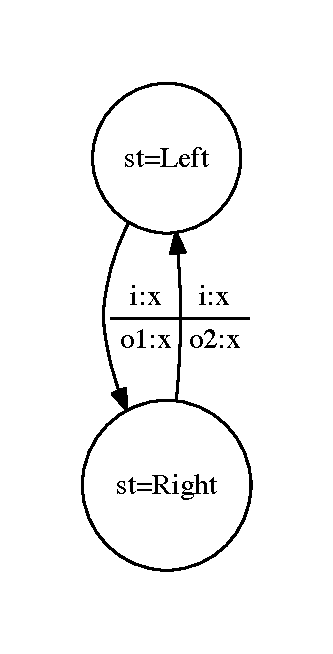
\includegraphics[height=7cm]{figs/switch-act-fsm}
  \end{minipage} \\
Program & FSM of the \texttt{switch} actor
\end{tabular}
  \caption{Example of FSM generation}
  \label{fig:switch-act-fsm}
\end{figure}
%$

\begin{figure}[h]
\begin{tabular}[c]{cc}
  \begin{minipage}[b]{0.5\linewidth}
    \begin{lstlisting}
actor suml
  in (a:signed<8> dc)
  out (c:signed<8>)
var st : {S0,S1} = S0
var s : signed<8>
rules
| (st:S0, a:'<) -> (st:S1, s:0)
| (st:S1, a:'p) -> (s:s+p)
| (st:S1, a:'>) -> (st:S0, c:s)
;

stream i:signed<8> dc from "sample.txt";
stream o:signed<8> to "result.txt";

net o = suml i;
    \end{lstlisting} 
  \end{minipage} &
  \begin{minipage}[b]{0.5\linewidth}
  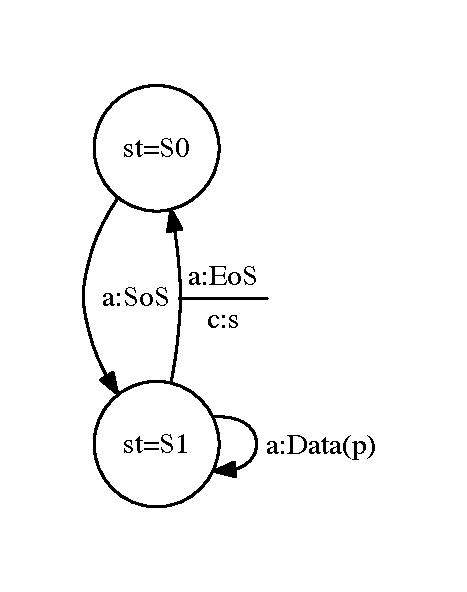
\includegraphics[height=7cm]{figs/suml-act-fsm}
  \end{minipage} \\
Program & FSM of the \texttt{suml} actor
\end{tabular}
  \caption{Example of FSM generation}
  \label{fig:suml-act-fsm}
\end{figure}
%$

\begin{figure}[h]
\begin{tabular}[c]{cc}
  \begin{minipage}[b]{0.4\linewidth}
    \begin{lstlisting}
actor sample (n: int)
  in (i: $t)
  out (o: $t)
var k : {1,..,n} = 1
rules
| i:x when k<n -> k:k+1
| i:x when k=n -> (k:1, o:x)
;
...
net o = sample 4 i;
    \end{lstlisting} 
  \end{minipage} &
  \begin{minipage}[b]{0.6\linewidth}
  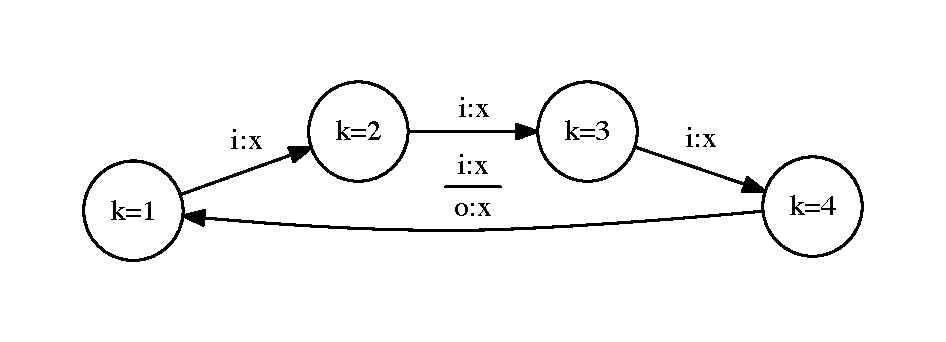
\includegraphics[width=1.0\linewidth]{figs/sample-act-fsm}
  \end{minipage} \\
Program & FSM of the \texttt{sample} actor
\end{tabular}
  \caption{Example of FSM generation}
  \label{fig:sample-act-fsm}
\end{figure}
%$

\section{The \texttt{caphmake} utility}
\label{sec:makefiles}

This utility, introduced in version 2.8.1, greatly simplifies the usage of the compiler by reducing
the configuration of a \caph project to the strict minimum\footnote{It can be viewed as the analogue
  of the \texttt{qmake} utility in \textsf{Qt} distributions.}.

Generating code and running simulations using the \caph compiler now proceeds as follows~:
\begin{enumerate}
\item generate a top-level Makefile by invoking \verb|caphmake|,
\item generate backend specific Makefiles by typing \verb|make makefiles|,
\item generate code and/or run simulations by invoking the ad-hoc rule; the most useful rules
  are\footnote{See the generated Makefiles for a complete list of rules.}~:
  \begin{itemize}
  \item \verb|make dot| to generate the \verb|.dot| representation of the program (\verb|make dot.show| to display it),
  \item \verb|make sim.run| to run the simulation using the interpreter (\verb|make sim.show| to display results),
  \item \verb|make systemc.code| to generate the SystemC code,
  \item \verb|make systemc.run| to generate the SystemC code and run the corresponding simulation (\verb|make systemc.show| to display results),
  \item \verb|make vhdl.code| to generate the VHDL code,
  \item \verb|make vhdl.run| to generate the VHDL code and run the corresponding simulation
    (\verb|make vhdl.show| to display results).
  \end{itemize}
\end{enumerate}

\medskip
The description of the \verb|caphmake| utility is provided in the appendices.

\medskip
Application-specific customization is essentially done by providing a file named
\verb|<app>.proj|, where \verb|<app>| is the name of the toplevel \caph source file
  (without the \verb|.cph| suffix),

  The \verb|.proj| file -- which must be placed in the same directory than the compiled program --
  essentially contains the values of the options to be passed to the compiler for each possible
  target\footnote{Technically, this file is simply included at the beginning of each of the
    Makefiles generated from the toplevel Makefile.} (\verb|.dot| generation, interpreter-based
  simulation, SystemC backend or VHDL backend). As an example, listing~\ref{lst:main-proj} gives a
  \verb|.proj| file which can be used for the testing the edge extraction application described in
  chapter 3 of the \caph tutorial ("Caph Primer").

\begin{lstlisting}[language=make,tabsize=4,basicstyle=\footnotesize,frame=single,caption={A possible 
    \texttt{.proj} file for the edge extraction application described in chapter 3 of the "Caph
    Primer"},label={lst:main-proj}]
GEN_OPTS = -D ifile=pcb.pgm -D threshold=80 
DOT_OPTS = $(GEN_OPTS)
SIM_OPTS = $(GEN_OPTS) -abbrev_dc_ctors -dump_channel_stats
SC_OPTS = $(GEN_OPTS) -sc_abbrev_dc_ctors -sc_stop_when_idle 1000 -sc_dump_fifo_stats 
VHDL_OPTS = $(GEN_OPTS) -vhdl_annot_file main_fifo_stats.dat
GHDL_RUN_OPTS = --stop-time=160000ns 
\end{lstlisting}

\medskip In some (rare) cases, the default targets produced in the target specific Makefiles when
invoking \verb|make makefiles| after \verb|caphmake| may not be adequate. A typical situation is
when some extra arguments, which cannot be guessed by compiler from the source code, have to be
passed to some utility programs. In this case, it is possible to override the corresponding rules by
writing a file \verb|<app>.rules| containing the new definitions\footnote{As for the \texttt{.proj}
  file, the \texttt{.rules} file must be located in the same directory than the compiled file.}.  As
an example, listing~\ref{lst:main-rules} gives the \verb|.rules| file which has been used for the testing
the second version of the edge extraction application described in chapter 3 of the \caph tutorial. 
Since this version makes use of centered convolution, \emph{blanking} parameters must be passed to
the passed to the \verb|pgm2bin| program when generating the \verb|.bin| input file from the input
\verb|.pgm| image. This cannot be guessed by the compiler and hence has to be specified in the
\verb|.rules| file\footnote{Technically this file is inserted at the end of the target specific Makefiles,
so that overriding can take places.  This explains why the corresponding definitions cannot
  be given in the \texttt{.proj} file.}.

\begin{lstlisting}[language=make,tabsize=4,basicstyle=\footnotesize,frame=single,caption={A possible 
    \texttt{.rules} file for the seconde version of the application described in chapter 3 of the
    tutorial},label={lst:main-rules}]
pcb.bin: pcb.pgm
	$(PGM2BIN) -hblank 4 -vblank 140 12 $< $@
\end{lstlisting}
%$

%%% Local Variables: 
%%% mode: latex
%%% TeX-master: "caph"
%%% End: 
